\section{The Zone of Innermost Desires}

\begin{wrapfigure}{rt}{.3\textwidth}
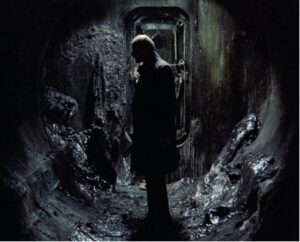
\includegraphics[width=.3\textwidth]{Stalker-300x242.jpg}
\end{wrapfigure}

You are sitting at the bus stop, or shopping at the outdoor market. A man who calls himself the Stalker hands you his calling card with his phone number and a mysterious, yet compelling, tagline. You complain about your malaise to a friend, who hands you the same card. Ultimately you don't know where or when you will meet the Stalker. Everyone will meet the Stalker sometime in his life. When that happens, he will be forced to make a decision.

The Stalker tells you of a place, a mysterious place called the Zone, that has a Room in which your most innermost desire is satisfied. The Stalker himself has no desire other than to lead others to it. He is poor and cannot provide adequately for his wife and disabled daughter. Like the final days of Siddhartha, he is just the ferryman.

The Zone is protected by armed guards who themselves fear the Zone. Once in the Zone, the Room is protected by traps, an eerie landscape, and tunnels. The Stalker demands absolute obedience in order to reach the Room safely. He warns of the fellow called the Porcupine who had reached the Room and then committed suicide.

Yet nothing deters you and the others in the small party you are with. The thought of fulfilling your innermost desire is too compelling. The trip to the center is the opposite of Lethe; instead of forgetting, one begins to remember. Are you mistaken about your innermost desire? Perhaps it is something else, because your desires conflict with each other.

Moreover, once your innermost desire is satisfied, it is no longer private. It is there for the world to see. Do you want your neighbors to know about your lusts for their wives of daughters? Or what you privately think about your family members? Your hatred for your boss, your envies, your greed? Wouldn't it be better to keep those to yourself? Perhaps you are not really the nice fellow you imagine yourself to be.

You reach the Room after many hardships. Instead of feeling the excitement of the imminent satisfaction of your desires, dread sets in. Maybe you don't really know your innermost desire as well as you had presumed. You don't want to be surprised. A Scientist in the party wants to blow up the Room so that no one can have his innermost desires satisfied; he rightly fears that.

Everyone leaves, unsatisfied.

\paragraph{Epilogue}

Most return to their ordinary lives in which nothing significant changes.

A very few encounter an esoteric school. There he learns ``the profound silence of desires, of preoccupations, of the imagination, of the memory and of discursive thought.'' (Valentin Tomberg)

He is no longer interested in satisfying desires since that is a passive exercise, something imposed on him from without. Instead, he develops a True Will.

\begin{quotex}
He who sees the beauty of that which he recognizes as true cannot fail to love it --- and in loving it the element of constraint in the duty prescribed by the true will disappear: duty becomes a delight. It is thus that ``work'' is transformed into ``play'' and concentration without effort becomes possible.
\flright{\textsc{Valentin Tomberg}}
\end{quotex}


Such a one is then free to fulfill the destiny given to him by Providence.

\textit{Stalker} Directed by \textbf{Andrei Tarkovsky}.

\url{https://www.youtube.com/watch?v=Q3hBLv-HLEc} 

\flrightit{Posted on 2022-05-15 by Cologero}

\begin{center}* * *\end{center}

\begin{footnotesize}
\begin{sffamily}
\texttt{Michael M on 2022-05-20 at 21:09 said:}

This is a film that contains a great deal of similarity to the work in Gnosis.

The Stalker in the film has to be followed even if the rational part of the characters tells them it doesn't make sense. Following conscious steps on the Way to a center that reveals an inner most desire, they realize the terrifying nature of the fallen personality. Something M. says all must do and accept within themselves to understand Reality as it is.

The Stalker laments at the end of the film as no one seems to understand, though many are called few answer and are willing to cross the next threshold.

\hfill

\texttt{AghorNath on 2022-05-23 at 23:36 said:}

Stalker, indeed every opus composed by Tarkovsky (at the behest of True Will), is/are mandatory viewing for those on the Straight Path... seeking the Narrow Gate. They are pensive, visionary recitals of initiation. Each film acts as a map through the veils of life, and plays out within the Alam al-Mithal, and it's varying degrees. They are prayers in motion.

The camera should always be viewed with the eye of the heart, mirroring His watchful eye.

Light a mental candle prior to every viewing, say a short pray. You might just get what you wish for!

\end{sffamily}
\end{footnotesize}

